\documentclass[msthesis.tex]{subfiles}
\def\Arrow{\raisebox{0.3\height}{\scalebox{2}{$\Rightarrow$}}}
\begin{document}

\chapter{Methods}
\begin{figure}

     \centering
     \begin{subfigure}[b]{0.4\textwidth}
         \centering
         \vspace{-2em}
         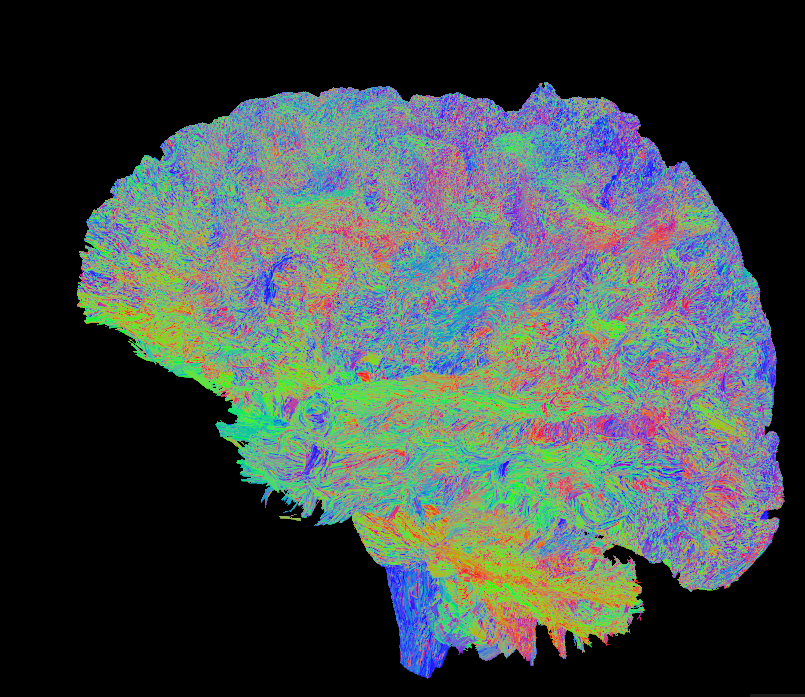
\includegraphics[height=0.9\textwidth,width=0.9\textwidth]{images/tractography.png}
         \caption{Tractography}
         \label{fig:1M_tract}
     \end{subfigure}
    \hfill
     \begin{subfigure}[b]{0.4\textwidth}
         \centering
         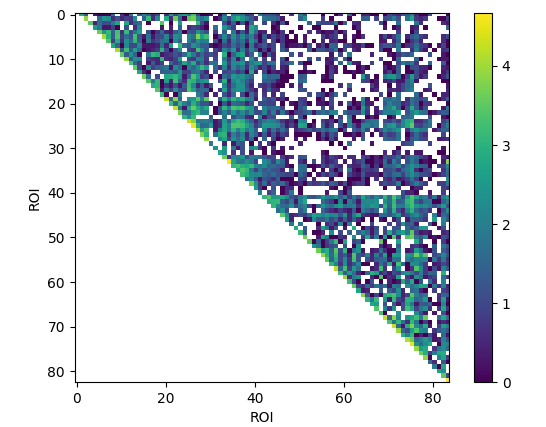
\includegraphics[height =0.9\textwidth,width=\textwidth]{images/connectome_1M.png}
         \caption{Connectome}
         \label{fig:connectivity_matrix}
        \end{subfigure}
    \vfill
        \begin{subfigure}[b]{0.6\textwidth}
         \centering
         \vspace{2em}
         %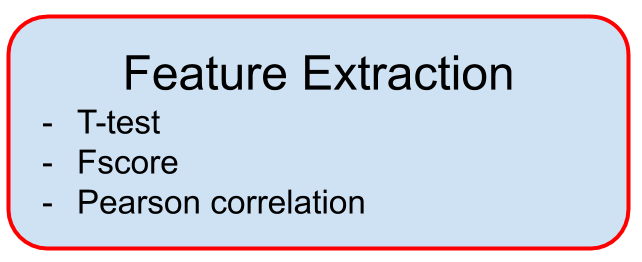
\includegraphics[height=0.3\textwidth,width=0.5\textwidth]{images/Features_1.png}
        \begin{tcolorbox}[box align= center,coltitle=black!75!black, colback=yellow!5!white,colframe=yellow!50!black,
  colbacktitle=yellow!80!black,title=\centering \large Feature Representation]
        \centering
        fscores, t-test, pearson correlation
        \end{tcolorbox}
        \caption{}
         \label{fig:feature extraction}
         \end{subfigure}
    \vfill
    \begin{subfigure}[b]{0.9\textwidth}
    \begin{subfigure}[b]{0.3\textwidth}
        \begin{tcolorbox}[coltitle=black!60!black ,colback=yellow!5!white,colframe=yellow!50!black,
  colbacktitle=yellow!75!black, fontupper=\color{black}, title=\centering \large Feature Selection]
        Select k\% features
        \end{tcolorbox}
         %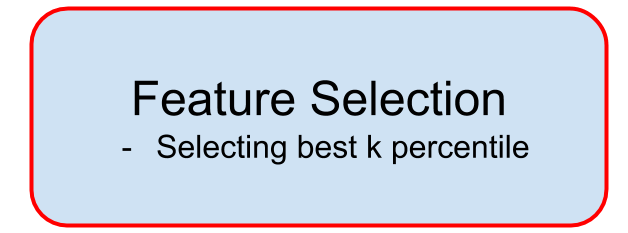
\includegraphics[height =0.8\textwidth,width=\textwidth]{images/Features_2.png}
         \vspace{+1.5cm}
         \label{fig:feature selection}
         \end{subfigure}
    \hfill
    \begin{subfigure}[b]{0.4\textwidth}
         \centering
         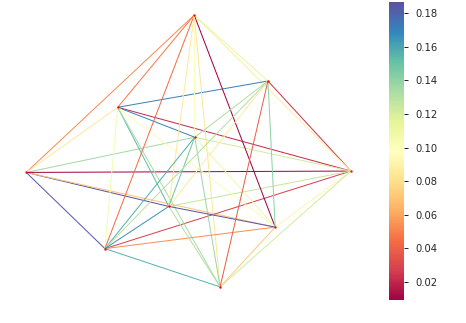
\includegraphics[height =0.8\textwidth,width=\textwidth]{images/mews.png}
         \label{fig:mewspip}
         \end{subfigure}
    \vspace{-2em}
     \caption{Parallel feature selection using baseline analysis and MEWS}
    \end{subfigure}
    \vfill
        \begin{subfigure}[b]{0.6\textwidth}
         \centering
         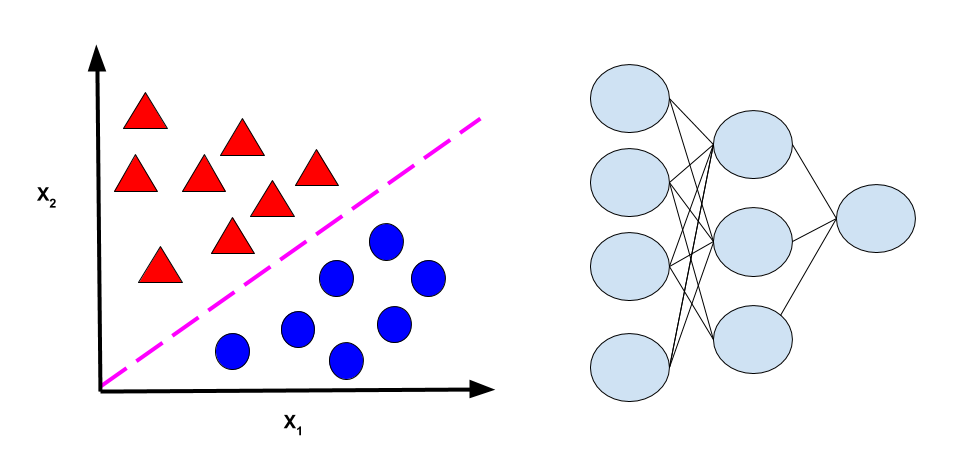
\includegraphics[height =0.4\textwidth,width=\textwidth]{images/classification.png}
         \caption{Classification}
         \label{fig:three sin x}
         \end{subfigure}
    \caption{(a) Whole brain tractography consisting of one million streamlines computed for each subject. (b) Connectivity matrix encoding DWI information. In this case, the matrix represents the number of streamlines between any two regions of interest in the $log_{10}$ scale. (c) Different statistical measures used to represent the importance of the original features present in the dataset.(d) Ranking used to determine the  most important features which are then fed to the classifier. Parallely, the MEWS is extracted from an input graph of statistical coefficients and is fed to the classifier (e) Classification using machine learning algorithms, such as SVMs, Random forests and MLPs.}    
    \label{fig:pipeline}
\end{figure}

A classification task on data from the Human Connectome Project was designed according to the pipeline presented in Fig. \ref{fig:pipeline}.  This pipeline consisted of four major steps. First, the whole brain tractography was first generated on the basis of DWI scans. Second,  a connectome was created and represented in the form of connectivity matrices. Two different feature selection techniques were deployed for classification of subjects based on the features in the connectivity matrices. Finally, these two techniques were compared based on classification metrics and the features they selected. 

The implementation of this pipeline was scripted in \textit{Python}. The preprocessing of the HCP data to generate tractography was done with the help of \textit{Mrtrix3}.  Data was prepared in a classification ready format using \textit{Pandas} (\cite{pandas_2020}) dataframes. The Maximum Edge Weight Subgraph problem was implemented in \text{Java} based on a modification from \cite{DBLP:journals/corr/LobodaAS16}. The final classification was based on machine learning from \textit{scikit-learn}(\cite{sklearn_2012}). 

\section{Data Acquisition}
\label{sec:acquisition}
Structural and Diffusion MRI for 203 subjects was acquired from the s900 release of the HCP (\cite{hcp2015wu}). Out of the total, 101 subjects were female and 102 were male. 83 females and 58 males were aged 26-30 and while the 34 male and 28 females were aged 22-25. The demographic information along with other markers about the subjects' emotion and cognition were obtained from the unrestricted access data available on \href{https://db.humanconnectome.org/}{\textbf{\textit{https://db.humanconnectome.org/}}}.


The structural and diffusion MRI files used for this project were obtained from the repositories containing volumes preprocessed using version 3 preprocessing pipelines of the HCP detailed in (\cite{GLASSER2013105}). A Siemens 3T Skyra system was used used to scan all subjects (starting in August 2012, housed at Washington University, St. Louis). The details of the acquisition protocol are mentioned in \cite{van2012human}.


There were two types of structural data required from the HCP pipeline for each subject in order to proceed with the task of the project. The first was a parcellation image consisting of a segmentation volume and a cortical surface parcellation based on the Desikan Killinay Atlas (\cite{desikan2006automated}), provided as a default in FreeSurfer). The second type was the T1w scan in subject space. This anatomical images was aligned to the location at the interface of hemispheres: the anterior commisure and posterior commisure (ACPC). It is a rigid body rotation so that the image gets 'centered', this process can be termed as registration.\iffalse This was a T1w volume data in the subject's native space obtained after rigid-body rotation to AC-PC alignment (rigidly aligned to the native axis of MNI space, also termed as registration )\fi. It was sampled at the same resolution as the diffusion data (1.25 mm isotropic, originally 0.77 mm isotropic).The parameters of the T1w images are presented in the table \ref{tab:structuralmri}.


\begin{table}[]
    \centering
    \begin{tabular}{|c|c|}
    \hline
         TR (ms) & 2400  \\
    \hline
         TE (ms) & 2.14 \\
    \hline
         T1 (ms) & 1000 \\
    \hline
         Flip angle & 8 deg \\
    \hline
         FOV & 224x224 \\
    \hline
         Voxel Size & 0.77 mm isotropic \\
    \hline
    \end{tabular}
    \caption{Acquisition parameters for the structural image acquisition from the s900 release. }
    \label{tab:structuralmri}
\end{table}

\begin{table}[]
\centering
    \begin{tabular}{|c|c|}
         \hline
         Sequence &  Spin-echo EPI \\
         \hline
         slice thickness & 1.25 mm, 1.25 mm isotropic voxels\\
          \hline
         TR (ms) & 5520  \\
          \hline
         TE (ms) & 89.5 \\
          \hline
         Flip angle & 78 deg \\
          \hline
         Refocusing flip angle & 180 deg \\
          \hline
         FOV & 224 x 224 \\
          \hline
        Voxel Size & 0.77 mm isotropic \\
          \hline
        b-values & 100,2000 and 3000 s/mm^2\\
         \hline
    \end{tabular}
    \caption{Parameters for the acquisition of the Diffusion MRI data acquired from the HCP.}
    \label{tab:diffusionmripara}
\end{table}

\subsection{Label Preparation}
\label{sec:label_preparation}
Different types of labels were used to test the method
Personality traits are based on the five factor model of personality. The five different personality traits are Agreeableness, Conscientuousness, Neuroticism and extraversion. They are often used in pyschology and pyschiatry to determine the behaviour of subjects
using questionnaires. The personality labels were continuous, their statistics in our dataset are depicted in table \ref{table:personality}
\begin{table}
\label{table:personality}
\csvreader[
  tabular=|c*{5}{|c}|,
  table head=\hline Variable & Agreeableness & Openness &  Conscientiousness &  Neuroticism  & Extraversion\\ \hline,
  late after last line=\\\hline,
]{tables/personality_traits_summary.csv}{}%
{\csvcoli & \csvcolii & \csvcoliii & \csvcoliv & \csvcolv & \csvcolvi}
\caption{Summary of personality traits for each different subjects}
\end{table}
Their conversion to the classification task were as follows
\begin{enumerate}
\item Record the median of the personality trait the training subjects
\item Divide the personality labels into 5 quartiles
 \item Remove the data of the subjects whose personality traits fall into the middle quartiles
 \item Binarize the variables such that the first two quartiles belong to the lower class and the last two quartiles correspond to the higher class
\end{enumerate}

The gender variables were categorical and for the classification task males were mapped to O and females to 1. 


\section{Creating the Connectome}

\begin{figure}
    \centering
    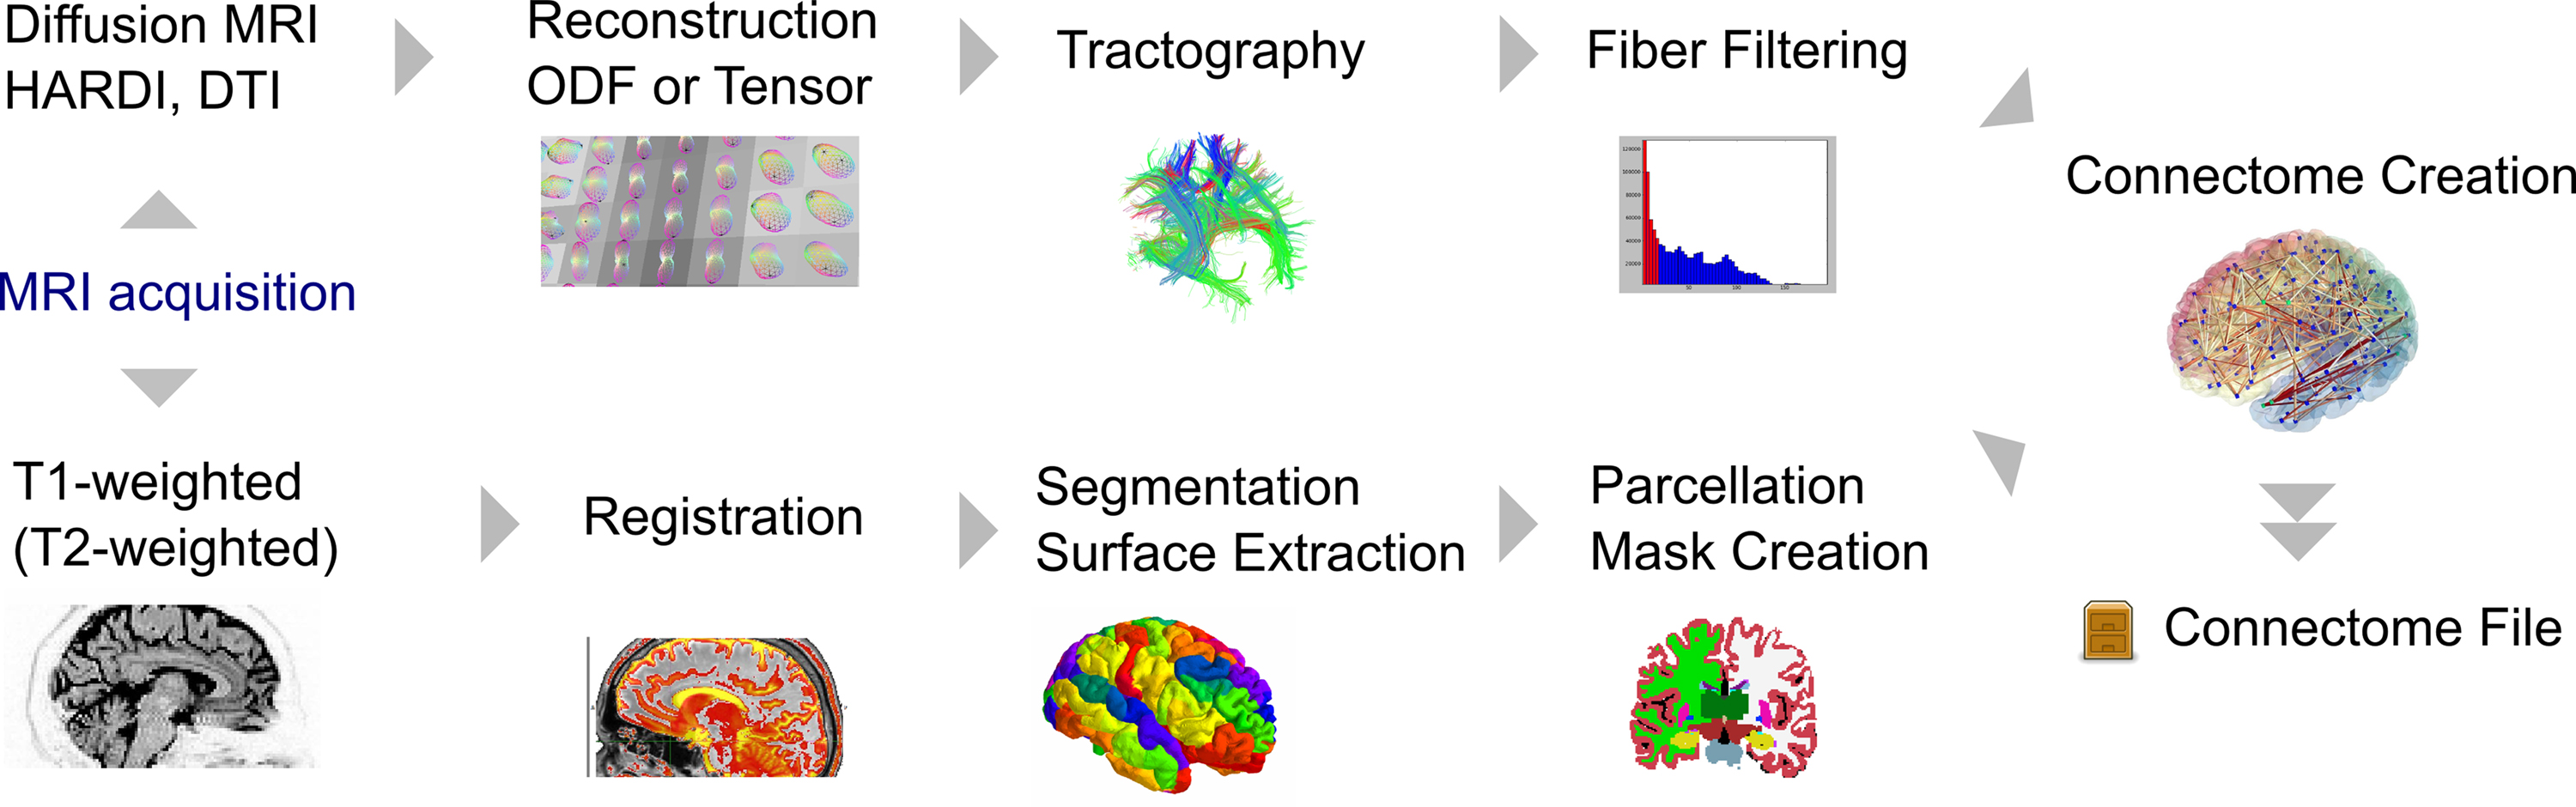
\includegraphics[width=\textwidth]{images/connectome_creation_workflow.png}
    \caption{Pipeline for creating the connectome for each subject. After the acquisition of the MRI data two parallel processes take place. The first parallel process is based processing the structural images for each subject in their native space. The second parallel process is the processing of the Diffusion data to generate Anatomically contstrained tractograms. After obtaining the fiber filtered tractograms and the parcellation masks with segmented tissues the connectome file is generated by determining the proprties of the streamlines that run between different ROIs.Image from \cite{gerhard2011connectome}}
    \label{fig:connectome_pipeline}
\end{figure}


For each subject, four types of  DWI files were used. First, the preprocessed diffusion time series file. Second, the brain mask in diffusion space. The other two types were diffusion weighting and diffusion direction for each volume. The important characteristics of the dMRI images is that they obtained in very high resolution (1.25mm isotropic) using a Stejskal-Tanner (monopolar) diffusion encoding scheme as mentioned in section \ref{sec:DWI}. The q-space was sampled by including 3 shells at the b-values presented in table \ref{tab:diffusionmripara} with each gradient table defined by a single b-value acquired once with right-to-left and another in the opposite phase encoding polarities. 

For this project, the structural images from subject's native space were taken due to the nature of the tractography. Tractography is performed in the subject space since a structural image in this space is the best approximation of the subject's physical brain. 



A connectome is generated on the basis of tractography as explained in section \ref{sec:connectomics}.The pipeline was implemented on the basis of the tutorial on Structural Connectome for Human Connectome from the software package \textbf{\textit{Mrtrix3}}. The preparation of the structural connectivity matrices can be visualized in the figure \ref{fig:connectome_pipeline} mainly involves three steps which are explained in the following subsections.

The structural and diffusion images available within the HCP data were used to prepare the data for probabilistic whole-brain tractography (\cite{parker2003framework}). the parcellation image was used to generate a volume delineating locations of the nodes of the connectome for each subject while the T1w image in a subject's native space were used to generate a five-tissue type segmented image.

\subsection{Structural Image Processing}
\label{subsec:struct_diff}

The first three steps of the structural image processing were readily accomplished by the HCP preprocessing pipeline. The segmentation surface was available from the HCP data as mentioned in section \ref{sec:acquisition}. However, the data obtained had a parcellation mask based on the default FreeSurfer segmentation which did not contain the numbering of the ROIs starting from 1. The parcellation mask was converted from FreeSufer's estimates of sub-cortical grey matter structures with the estimates from FSL's FIRST tool. This made the numbering of the ROIs (also the nodes in this case) from 1. 

In addition to creating the parcellation mass, a five tissue segmented image (5TT) was also generated. This was done on the basis of the T1w structural volume mentioned in \ref{sec:acquisition} sampled at the same resolution as the diffusion data (1.25 mm isotropic). The 5TT image contained differentiation of brain regions into five tissue types, namely subcortical white matter, WM, cerebrospinal fluid (CSF) and optionally pathological tissue. The segmentation is based on FSL segmentation tools FIRST and FAST.This information about the location of different tissue types makes the tracking based on DWI images suitable for Anatomically constrained tractography.  (\cite{anattractsmith}). 


\iffalse
The diffusion image was first converted to a non-compressed format. The information about the diffusion gradient encoding was represented in the header of the file, the volume data was made continuous voxel-wise and the data points were converted to a floating point format. 
After this, the mean b=0 image was generated for visualization. The b=0 image serves as a sort of baseline for anatomical reference.

The multi-shell, multi-tissue response function was determined  in order to form Multi-Shell, Multi-tissue spherical deconvolution. 

Atleast three unique b-values are required to estimate three tissue comparments. These 

The deconvolution leads to the formation of a 4 dimensional image in which each 3D volume (as viewed in \comment{part of pipeline figure in preprocessing} is RGB encoded where the cerebrospinal fluid (CSF) is seen in red, the gray matter in green and the white matter in blue. 
\fi

\iffalse
In order to prepare for the tractography, the structural T1w images were preprocessed by Dr. Regina Wehler during the course of her master's thesis. At first the five-tissue-type images were generated using the 5ttgen fsl command. These are segmented 4D images whose fourth dimension represents 5 volumes containing the partial fractions of cortical gray matter, sub-cortical gray matter, white matter, CSF and pathological tissue. 
The input files were converted from the nifti to the mif format using the mrconvert command for the data to be compatible with \textbf{\textit{Mrtrix3}}. Then the 5TT images were generated using the 5ttgen fsl command -nocrop option to keep the images at the size of the original input. 
After obtaining the 5TT images, the segmentation from the original FreeSurfer format were converted to the scheme of the Desikan Killiany Atlas(\cite{desikan2006automated}) which divides the human cerebral brain into gyral based regions of interest.
\fi

\subsection{Diffusion Image Processing}

The first step of processing the diffusion images is to determine the fODF for probabilistic tractography. The fODFs were reconstructed using multi-shell, multi-tissue constrained spherical deconvolution (MSMT-CSD) based on the algorithm in \cite{jeurissen2014multi}. As mentioned in section \ref{sec:highermodels} the CSD of response functions can determine the fODF distribution. Hence, CSD of the separate response functions from WM, GM and CSF was done in order to obtain the DWI signals of the three tissue types from the 5TT image.

The probabilistic whole-brain tractography of five-million fiber tracts was generated using \textbf{\textit{Mrtrix3}} (\cite{tournier2019mrtrix3}). The streamlines were computed on the basis of the algorithm iFOD2 (\cite{tournier2010improved}). This algorithm uses the fiber orientation Distribution (fODF) image and determines candidate streamline paths (arcs), which have greater fODF amplitudes along the paths. By sampling the underlying fODF amplitudes along these arcs , it makes the streamlines likely to follow most probable paths.

Anatomical constraints on the tractography were provided using the five tissue type image. There were other series of constraints imposed in order to make the  tractography more informed. The seed points were dynamically determined using the Spherical-deconvolution informed filtering (SIFT) model \cite{smith2013sift} of the white matter fODFs. The cutoff value of 0.06 was set for FOD amplitude for terminating tracks. The maximum length of streamlines was set at 250 mm (200 times the voxel size) when the voxel size is 1.25mm. The tracking along a streamline was truncated if the fiber terminates at poor structural, then  retracking is performed. The streamlines were cropped whenever as the streamlines cross the grey matter-white matter interface. 

The tractography was then downsampled from five mullion fibers to one million fibers to preserve the most biologically relevant fibers using the SIFT algorithm (\cite{smith2013sift}). This provides more meaningful estimates of the structural connection density and also reduced the memory requirements. 
\iffalse
\begin{figure}
    \centering
    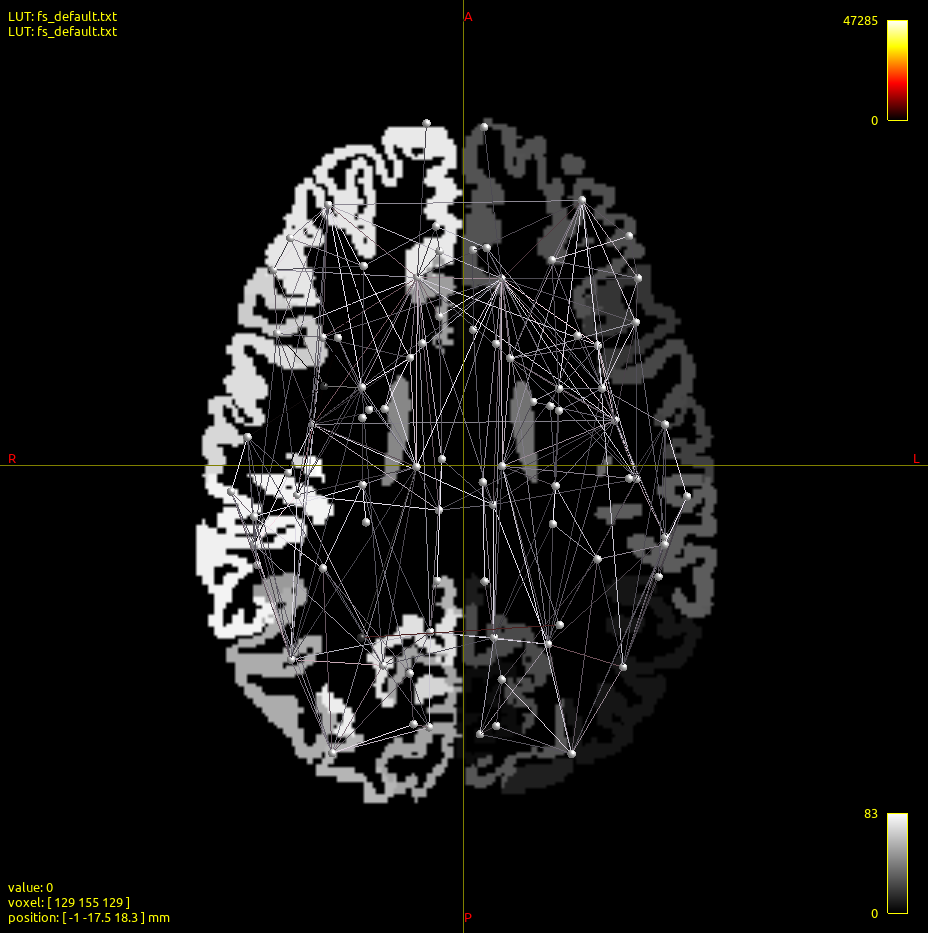
\includegraphics[width=0.8\textwidth]{images/connectome.png}
    \caption{Caption}
    \label{fig:connectome_vis}
\end{figure}
\fi
\subsection{Connectome Generation}

The connectome can be represented in the form of a graph as mentioned in section \ref{sec:connectomics}. After obtaining the streamline file and a parcellation image representing the subject specific node locations of the connectome, the connectome matrix was obtained in a .csv format. It was generated from the whole brain tractography of one million tracts using 84 relevant grey matter parcellations (in \textit{\textbf{Mrtrix3}}) from the default FreeSurfer segementation specified by the Desikan Killiany Atlas. 

Using different parameter settings three types of features were extracted. The mean fractional anisotropy (or mean FA, equation \ref{eq:meanFA}), of the streamlines that connect the two regions. The average length of streamlines connecting two regions and number of streamlines between any two regions. The visualization can be seen in the Fig. \ref{fig:connectivity_matrix}. The connectome is represented as an upper triangular matrix($84 x 84$) considering that the connections between two ROIs are symmetric.

\iffalse
In the Fig. it can be seen that there is a need to decipher the streamlines which are terminating in the specified regions of interest
\fi
\section{Feature representation}
Once the connectivity matrices for all the 201 subjects were computed and encoded in the format of a .csv file, a \textit{pandas} dataframe was prepared in order to be prepared to fit into the classifier. Each row represented the data for an individual subject. Each column represented the connection between any two brain regions i.e. features in one cell of the connectivity matrix. Three different types of features obtained using the connectome files as per \ref{subsec:connectome_generation} were kept structured to be separate so that at any time only the same type of features are used to be filtered.The exact structure varied according to the feature selection techniques employed.

Self-loops were omitted from the analysis pipeline due to incompatibility with the solver based implementation and non-significant changes to classification accuracy based on the omission. Further, using the calculation of statistical coefficients on the raw data the importance of each feature was determined.

The training set consisted of 141 subjects consisting of 83 females and 58 males aged 26-30. While the independent test set consisted of 34 male and 28 females aged 22-25. 

\subsection{Exclusion of self loops}
\label{sec:exclusion}
Self loops are considered the connections from the brain regions to themselves. They were excluded from the analysis in the very beginning. On the basis of performance of the classifiers it was seen that without the self loops the performance the classifiers still perform almost similarly.

To see the difference in between the classification accuracies, a paired sample t-test was conducted. In this t-test the paired samples are the classification metrics in the dataframe including the self loops and excluding them. The null hypothesis of this two-sided t-test was that the average of a particular classification metric on the basis of one feature (such as mean FA, mean streamline length etc.) with respect to five different personality traits was identical.
\begin{align}
    \label{eq:pairedtest}
    t = \frac{\Tilde{X_{D}} - \mu_0}{\frac{s_{D}}{\sqrt{n}}} \\
    \Tilde{X_D} = \sum_{i=1}^{N} \frac{a_{i} - b_{i}}{n}
\end{align}
where $s_D$ is the standard deviation of the differences between the metrics of the experiments with the self loops $a$ and without the self loops $b$. 

The null hypothesis could not be rejected because for the test data, the p-values of these t-tests was high and hence not corresponding to any statistical significance. The results of this experiment are presented in section \ref{res:selfloops}. 
\iffalse
avg mean FA for all self loops(along all subjects in training data) 0.36
avg mean FA for all the other areas without the self loops (across all the subjects) is 0.345 (avg)
max avg mean FA in the range is 0.66 (in one connection avg along all subjects)
\fi

\subsection{Statistical Coefficients}
\label{subsub:statcoef}
\iffalse
Three different metrics were used to filter the features. Namely, pearson correlation coefficient, f-scores and the p-value of the t-test. The pearson correlation coefficient for the continuous values of the different personality traits, while the f-scores and t-test calculations were based on the conversion of the continuous variables into classes according to the section \ref{sec:label_preparation}. 
\fi
Statistical coefficients were determined to be one of the most important feature filter methods for the classification from Neuroimaging data. Filter methods were used since they do not compromise on interpretability of the results.

Three different statistical coefficients were used mainly. The first two were the t-test and the fscore, based on the discriminative power of a particular feature. The pearson correlation coefficient was used to determine the relationship between the continuous output variable values and the feature values. 

The fscore used in the analysis is used to measure how well the particular feature distinguishes between the two classes labelled as 1 and 2. It  was calculated according to the equation \ref{eq:fscores}. 

The t-test was processed in a different manner as compared to the first two metrics, the training data was divided into two groups, one belonging to class 0 and the other belonging to class. The null-hypothesis remained that the means of the given feature for the two samples are identical i.e. $\overline{x_{1}} - \overline{x_{2}} = 0$. The p-value of the t-test was used to determine it's statistical significance by converting it into the $log_10$ scale. Each p-value $p_x$ was represented by $ f(p_{x}) = (-1)*\log_{10} p_x$ so that a higher numerical value represents a higher statistical significance.



\subsection{Feature selection} 
There were two types of feature selection techniques used before classification. The first represents a classical feature selection technique based on statistical coefficients while the second is based on extracting a subgraph after converting the original edge weights to statistical coefficients. The Maximum edge weight subgraph technique adds additional information about the graph topology. 

The hypothesis remained that the MEWS technique produces more interpretable results as it is based on it's connectedness constraints. The motivation to implement subgraph extraction methods is the fact that analyzing the inter-subject differences at the subnetwork level is much more easier than analyzing dense subgraph of whole brain connectivity. 

\subsubsection{Baseline analysis}
% Question: which one do we report? Solver was working only with the pearson correlation coefficient.

Baseline experiments were based purely on the filter methods mentioned in section \ref{subsec:filtermethods}. In this technique, there is no information about graph topology, the biological correspondence of the data and its logical expectations. It is based purely on numerical artefacts. 

For each of the structural connections, the statistical coefficient was calculated based on the data and target variables from the training set. The metrics mentioned in \ref{subsub:statcoef} were then used to rank the features. This ranking was based on first taking the absolute value of the coefficients and then dividing the coefficients for all features into percentile. This gave a ranking from which the top percentiles were selected top percentiles.

In our analysis we wanted to cover a range of number of features to cover overall trend of changes in metrics. Computational expense, the percentage of features to be chosen and compared was 2,5,10,50,100. With this range of percentages it could be determined how the metrics changed as a function of the percentage of features.


\iffalse
The pearson correlation coefficient was computed between the values of the feature for the training subjects and their corresponding personality trait values. It was a trial to capture the linear relationship between a parameter (eg. mean FA) representing a brain connection and the outcome label (i.e. personality trait).

The fscore based selection was done by computing the fscore between the feature values for the training set and thresholded values of the target variables according to the median of the training data labels. 

The fscores served as feature filtering step for the baseline experiments as they were used by dividing the f-score distribution into percentiles and then choosing the percentage of features we want in the specified top percentile. However, for the solver based experiments the fscores for each feature was (numerically) low which made the MIP problem hard to run computationally. Even multiplying the f-scores with an order of $10^3$ was not useful since the standard deviation of the f-scores was not too high (insert the standard deviation). 

This feature selection was in fact quite useful for the feature selection in the baseline experiments. The p-value of the t-test could be divided into percentile distributions and the top percentiles could be chosen accordingly. However, for the solver based experiments this selection did not work well due to computational effort. 

The pearson correlation coefficient in fact did work because it considers the linear nature of the personality trait coefficients. This type of feature selection is well reported in literature for Neuroimaging data considering continuous variables. It performed well for the baseline experiments as well as the solver based feature selection. For both the cases the absolute value of the pearson correlation coefficient was taken because only the correlation was important, whether it is positive or negative correlation was not a matter of concern for the analysis.

The f-score and the t-test were based on the binarization of the target variables according to the median values of the feature from the training set, this might lead to information loss and hence their lower numerical values. 
\fi

\subsubsection{Maximum Edge Weighted Subgraph}
\label{method:MEWS}

The special case of the MCWS, the MEWS was implemented because of no predefined node weighting for the regions of interest. The implementation was based on  the Java application from \cite{DBLP:journals/corr/LobodaAS16}. This application made use of the IBM ILOG CPLEX studio version 12.10 Java API. 

The input graphs implemented for the use-case were created after determining the statistical coefficients. The nodes in the graph consisted of 84 nodes defined by the cortical parcellations based on the Desikan Killiany Atlas. 

The edges represent the numerical values obtained from the feature extraction using statistical coefficients. The nodes were given a constant negative weighting of $-0.01$ to assure a negative penality on the inclusion of an extra node, this made the conservation of a specified number of nodes possible. Additionally, sparsity to the input graph was introduced using two constraints. The first being that the absolute value of the edge weights shall not be zero and that features are conserved if and only if the tractography of each subject contains atleast one streamline between the two nodes. 

An object oriented approach was taken to impalement a class derived from the \textit{networkx} graphclass for the different input and output graphs. Each input graph had a corresponding output graph. 
\iffalse
Nodes could be given different types of weighting such as the maximum of the incoming edge weights, any numerical constant or the average of the incoming edge weights. Further the edges could be filtered on the basis of thresholds for the numerical features.
\fi
The output number of edges is a function of the number of nodes. The output representing the number of edges as a function of nodes is presented in the results section (). 

For creating the output graph parts of the pipeline \cite{DBLP:journals/corr/LobodaAS16} were modified. Constraints mentioned in \ref{sec:MEWS} were extended. The additional constraint was 
\begin{align}
    \label{eq:sum_constraints}
    \sum_{v=1}^{V} y_v = m        &&  \forall v \in V
\end{align}
where m is a controllable parameter specifying the number of nodes needed to be preserved in the output graph and $y_v$ is the binary variable mentioned in equation \ref{eq:y_v}. The preprocessing workflow of the MCWS Java solver was disabled due to it's incompatability with our required constraint of preserving at most m nodes in the output graphs.


\section{Supervised Classification}

\subsection{Classification}
A Randomized Search cross validation with implementation from \textit{scikit learn} was carried out for different algorithms.After the randomized search was finished, the best estimator was taken and fit to the training set. This classifier was then used to make preductions on an independent test set with difference in age range.

One model was trained each time there was a different configuration of settings. The configurations were 

The classification metrics used were area under the curve, f1 score, accuracy and balanced accuracy.  
\begin{itemize}
    \item Support Vector Machines
    \item Random Forests

\end{itemize}


\section{Visualization}


\end{document}

